\section{数値解析例}
本節では,Na型モンモリロナイトに対する水和エネルギーを用いて行ったCG-MD
シミュレーションの結果を示す.
CG-MD解析では,温度,相対湿度,圧力を一定に保った状態で非平衡状態にある
初期モデルから,モンモリロナイト含水系(以下,粘土含水系と呼ぶ)の
CG-MDモデルで緩和計算を行う.
これを6つの異なる相対湿度において行い,膨潤挙動の観点からみたときの,
シミュレーション結果の妥当性について議論する.
以下,初期モデルと計算手順を述べた後,シミュレーション結果を
粘土分子配置のスナップショットと層間距離の頻度分布を示す。
これらの結果をもとに,相対湿度に応じた膨潤状態の変化について述べる.
\subsection{計算手順}
緩和計算を行うための初期モデルを図\ref{fig:fig3}-(a)に示す.
これは,2021年度の共同研究報告書で述べた方法で得た粘土含水系
モデルの一つで,粗視化粒子数は3,194で80の粘土分子からなるも
のである.このモデルを得た手順は以下の通りである.
はじめに,直線状の粘土分子を200$\times$200[nm$^2$]の
矩形領域に互いに重ならないよう,位置と向きをランダムに配置する.
次に,この系を周期構造を構成する単位セルとして用い,
乾燥密度が約1.6g/cm$^{3}$となるまで1[ns]かけて断熱圧縮する.
このとき,粒子系の運動方程式を時間積分するための時間ステップ幅
は0.02[ps],時間ステップ数は5万ステップとしている.
時間積分に関するこの条件は,以後の解析でも同じである.
断熱圧縮過程では系の温度を制御していないため,圧縮によって系に加えれられた
エネルギーで非常に高い温度にあり,平衡状態にも無い.
そこで,圧縮後のモデルを300Kまで$250$psをかけて冷却し,
その後750psの間一定温度(300K)で緩和計算を行う.
なお,緩和とは,温度や体積などの外的条件を一定にして,
系を平衡状態に向けて推移させることを意味する.
ここまでの計算では,水分量は各粗視化粒子において,水分量を表す
パラメータを二層膨潤状態に相当する$\sigma=1.5$[nm]に固定し,
系内での水分移動も系外との水分の授受もないものとしている.
最後に,無次元化された化学ポテンシャル$\bar \mu$を$0.5$に保ち,
温度と体積一定の条件で水分量を含めた緩和計算を1[ns]間行う.
$\bar \mu$の値は,強い排水が起こるように設定されており,
その緩和後は大きな層外空隙をもつ組織構造が得られる.
図\ref{fig:fig3}-(a)は以上の手続きによって得た粘土含水系モデルである.
これを初期構造として用い,Na型モンモリロナイトの水和エネルギーモデルを用いた
ときに,相対湿度に応じてどのような組織構造へ移行するか調べる.
なお,初期構造を得るための計算では,昨年度の共同研究で検討を行った
水和エネルギーモデルの一つである振動モデルを用いている.
これは仮想的な粘土の水和挙動を表現したもので,今回新たに
作成したNa型モンモリロナイトを対象としたものとは異なる.
そのため,初期構造は今回用いる水和エネルギー関数の元では平衡状態になく,
相対湿度の設定によらず,水分や分子配置に関して程度の差はあれ
必ず何らかの変化が生じる.

以下,温度を300K, 圧力を10MPaとして,いくつかの相対湿度で平衡化計算を 行い,どのような膨潤状態が現れるかCG-MD計算の例として示す. 

なお,冷却と緩和の間も水分量は2層膨潤状態で固定している.
図\ref{fig:fig3}(d)は,以上の結果として得られた状態を示す.
ここで(c)と(d)の図を見ると粘土分子の配置にはほとんど差がない.
これは,冷却によって粗視化粒子の振動は抑えられるが,密度が高く粒子位置は
ほとんど変化を起こすことができないためである.

\subsection{追加したテキスト}
図2
湿度を指定して行った,Na型モンモリロナイトの膨潤シミュレーション.(a)は粘土含水系モデルの初期状態を,(b)は相対湿度50$\%$, 
(c)は 相対湿度75$\%$において緩和計算を行い最終的に得られた組織構造(粘土分子配置)のスナップショットを示す.

(a)に示した初期状態は2021年度共同研究で得られた,仮想的な粘土の組織構造モデルである.
このモデルでは系全体が一層膨潤に達するには不十分な水分量しかもたない,乾燥状態に近いモデルになっている.
これを始状態とし,相対湿度をそれぞれ50$\%$および75$\%$に設定し,温度を300で一定として組織構造の緩和(平衡化)
計算を行った結果が(b)と(c)である.いずれもの場合も吸水が起こり,粘土層間距離が拡がっている.
その結果,粘土分子の積層体は顕著に体積が増す一方,粘土層外の間隙が積層体の体積増加を吸収するためにモデル全体の膨潤量は小さい.
湿度75$\%$のケースでは50$\%$に比較して吸水量が大きく,積層体の体積膨張もより大きいため,層外の間隙がほとんど消失していることが分かる.

図3
湿度を指定して行ったNa型モンモリロナイトの膨潤シミュレーションの結果.
(a)は初期状態,(b)は相対湿度50$\%$, (c)は 相対湿度75$\%$における粘土層間距離の頻度分布を示す.

初期状態(a)では層間距離が11〜12Åの範囲にあり0層から1層膨潤状態への中間にある.
この状態から相対湿度を50$\%$にして緩和計算を行った結果である(b)では,層間距離は12.5Å近傍に集中し,
ほぼ1膨潤状態のみとなっている.さらに相対湿度をあげた75$\%$では,13.2$\AA$と15.5$\AA$付近に2つのピークを持つ頻度分布となっている.
頻度分布の前者のピークは,1層から2層膨潤へ移行する直前の,後者のピークは2層膨潤状態の層間距離に相当し,
このケースでは1層と2層膨潤状態が混在することを示している.
いずれの相対湿度も,図1-(a)に示したXRD試験で観測される層間距離と近い値であることがわかる.
このことからも,本研究で用いた水和エネルギーモデルには,観測で得られたNa型モンモリロナイトの膨潤特性が反映されていることが確かめられる.
%--------------------
\begin{figure}[h]
	\begin{center}
	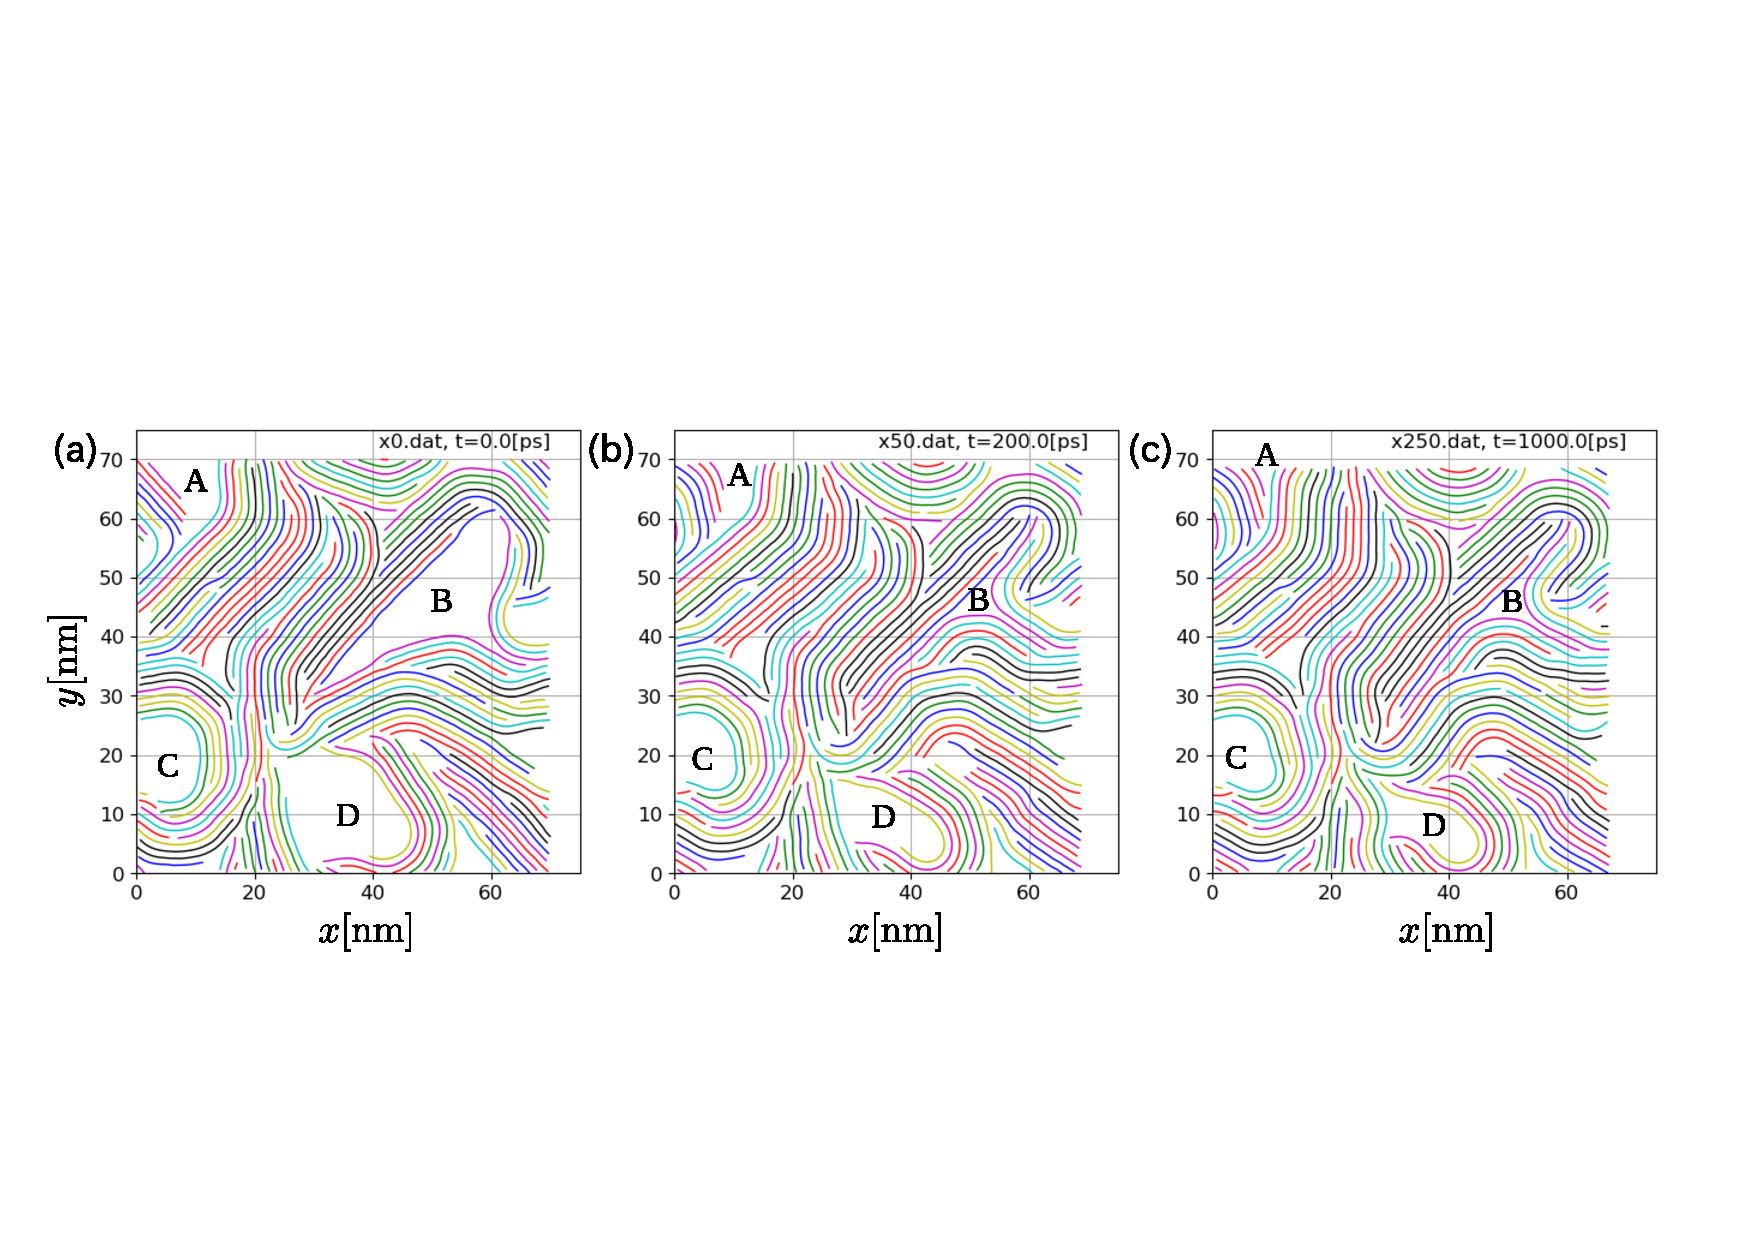
\includegraphics[width=1.0\linewidth]{Figs/fig3.pdf} 
	\end{center}
	\caption{
		caption.
	} 
	\label{fig:fig3}
\end{figure}
%--------------------
\begin{figure}[h]
	\begin{center}
	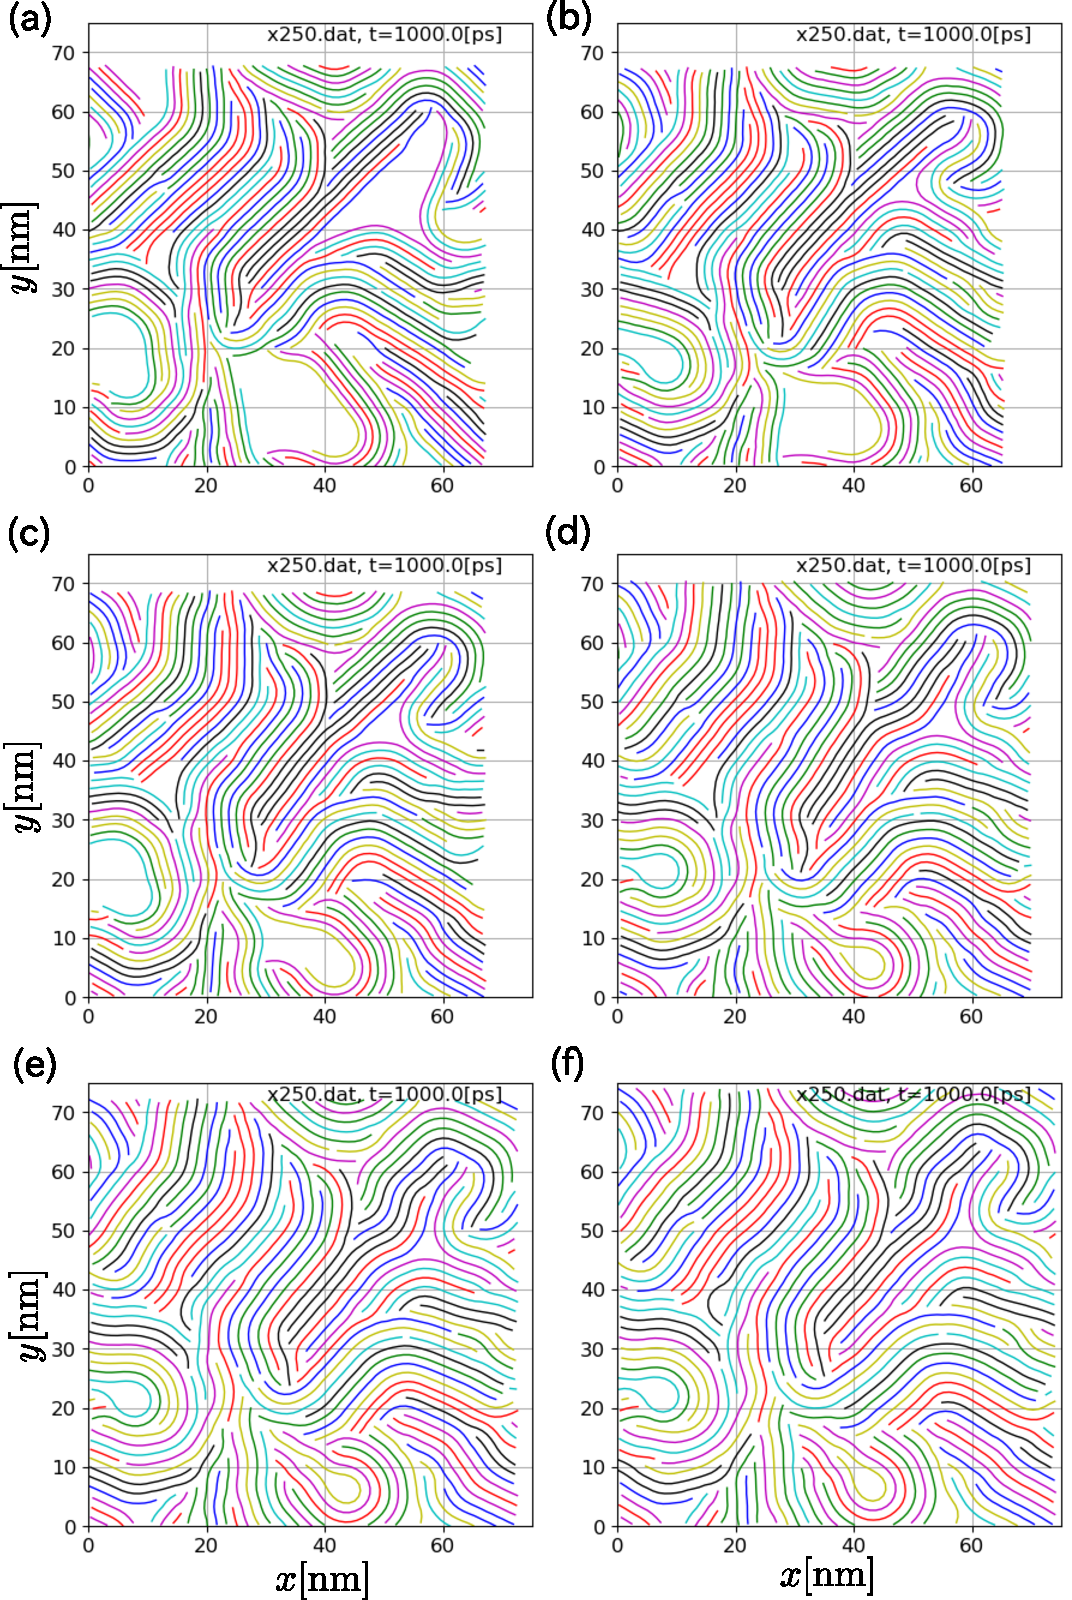
\includegraphics[width=1.0\linewidth]{Figs/fig4.pdf} 
	\end{center}
	\caption{
		caption.
	} 
	\label{fig:fig4}
\end{figure}
%--------------------
%--------------------
\begin{figure}[h]
	\begin{center}
	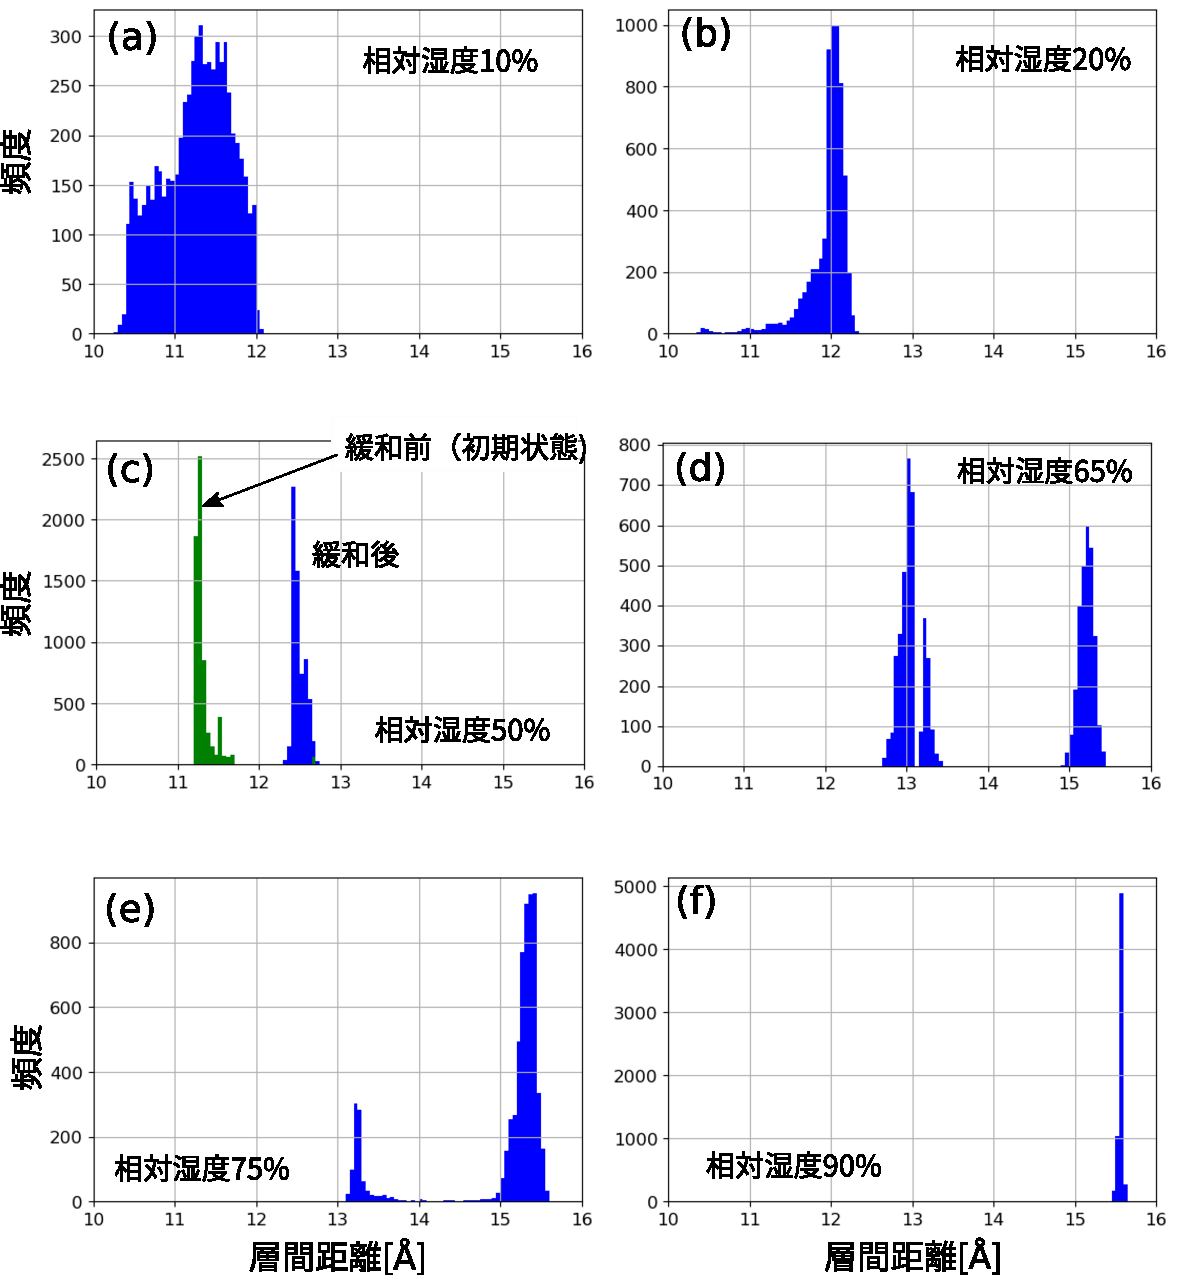
\includegraphics[width=1.0\linewidth]{Figs/fig5.pdf} 
	\end{center}
	\caption{
		caption.
	} 
	\label{fig:fig5}
\end{figure}
%--------------------
%--------------------
\subsection{化学ポテンシャル一定での平衡化}
%	図4 :化学ポテンシャル一定での平衡化 図4
次に,図\ref{fig:fig3}(d)を新たな初期状態として,体積,温度,
化学ポテンシャル一定の条件で緩和計算を行い,別の平衡状態へ推移させる.
このとき,指定された化学ポテンシャルに応じて粘土含水系は吸排水し,
水分の総量や膨潤状態が変化する.
また,水和エネルギーモデルには振動モデルを用い,水和エネルギーの大きさ
を規定する式(\ref{eqn:us_triwv})の$u_{\infty}$は,緩和開始時の
相互作用ポテンシャル$\left. U_{LJ}\right|_{t=0}$に対して,
\begin{equation}
	u_{\infty}=5\frac{\left.U_{LJ}\right|_{t=0}}{N_p}
	\label{eqn:uinf_val}
\end{equation}
とした.ただし,$N_p$は粗視化粒子の数を表す.
$u_{\infty}$は無限膨潤状態での水和エネルギーの大きさであるため,式(\ref{eqn:uinf_val})は,
水和エネルギーが最大で粒子あたりの相互作用エネルギーの5倍になるということを意味する.
一方,化学ポテンシャル$\tilde \mu$は単位長さあたりのエネルギーの次元を持つ.
そこで,
\begin{equation}
	\bar \mu = \frac{\tilde \mu }{\gamma u_{\infty}}
	\label{eqn:mu_bar}
\end{equation}
と無次元化する.$\gamma$は,単調成分(\ref{eqn:u_s})の減衰率で長さの逆数の次元
をもつ.また,規格化定数である$\gamma u_\infty$は,単調成分の
$s=0$での勾配という物理的意味をもつ.以下,化学ポテンシャルの大小は
式(\ref{eqn:mu_bar})の$\bar \mu$で表す.

図\ref{fig:fig4}は化学ポテンシャルによる影響をみるため,
$\bar{\mu}=0.1, 0.3$および$0.4$で1ns間,緩和計算を行った結果を
示したものである.この図の(a)は,緩和開始時の粘土分子の配置を,
(b)-(d)は各々の図に示した無次元化化学ポテンシャルに対する
緩和後の状態を示す.(b)と(c)のケースでは緩和開始時点から顕著な変化がみられない.
これに対して(d)では明らかに空隙が拡大している.化学ポテンシャルの逆数は
粘土含水系が置かれた環境の湿度指標と考えてよく,大きな$\bar{\mu}$は低い湿度に相当する.
そのため(d)では顕著な排水が起き,結果として層外の空隙が拡がっている.
(a)や(b)と比べると,(c)でも若干の空隙の拡大は認められるが,
図\ref{fig:fig4}だけからでは排水の結果であるか否かは判断し難い.
%	図5 :エネルギーの推移(化学ポテンシャル0.3の場合)
そこで,緩和途上でのエネルギーの変化を調べると図\ref{fig:fig5}のようになっている.
このグラフは,水和エネルギー$U_{hyd}$, 水分量に関するエネルギー$U_{N}$,
相互作用ポテンシャル$U_{LJ}$とそれらの和である全エネルギー$E$を示したものである.
このうち,系内に含まれる水分の増減は$U_{N}$の変化で示され,水分が増加(減少)するとき
$U_N$も増加(減少)する.
図\ref{fig:fig5}では,緩和の開始とともに$U_{N}$が減少して一定値に収束し,
当初よりも水分量が減少,すなわち排水が生じていることが分かる.
なお,水和エネルギーは最終的には当初より増加するが,
相互作用ポテンシャルは排水によって粒子間の相互作用が弱まり減少している.
以上の結果,全エネルギーは当初よりも小さな値に収束していることがこの図
に示されている.

%	図6 :水和水層厚のヒストグラム
% 山や谷の位置を参照するための記号を図中に書き入れること
次に,図\ref{fig:fig4}に示したそれぞれの状態が,どのような膨潤状態にあるか調べる.
そのために,水和水層の厚さ$s$の頻度分布を図\ref{fig:fig6}に示す.
水和水層の厚さ$s_i^\pm$は各粗視化粒子の上下方向で求められる.粗視化粒子数は
$N_p=$3,194個だから,図\ref{fig:fig6}は$N_p\times$2=6,388の
サンプルからなる頻度分布で,水和層の厚さに関する頻度(度数)の正規化等
を行わず,そのまま示している.
図\ref{fig:fig4}(a)の緩和開始時点では,全ての粒子の上下方向とも2層膨潤状態
に固定されている.そのため,水和水層の厚さは一律0.3nmで頻度分布はこの位置に
集中し(図\ref{fig:fig6}(a)),緩和終了時には指定された化学ポテンシャルに
応じて分布形が変化する.図\ref{fig:fig6}(b)の$\bar{\mu}=0.1$の場合,
ヒストグラムはほぼ一つの水和水層厚に集中した状態が維持されているが,
層厚は0.3から0.28nm程度に低下している.このことは,わずかに排水が生じ,
ほぼ単一の膨潤状態をとることを意味する.$\bar{\mu}=0.3$では,
同様な傾向の変化がよりはっきりと頻度分布に現れている.すなわち,
水和層の厚さがおよそ0.25nm程度まで低下し,分布幅が当初よりも大きくなるが,
依然として狭い範囲に集中している.
これに対して,組織構造に顕著な変化が現れる$\bar{\mu}=0.4$のケース
(図\ref{fig:fig5}(d))では,2つのピークをもつ頻度分布となっている.
これは,排水により2つの膨潤状態に分離することを示し,
単調な水和エネルギーモデルを用いた場合には現れない挙動である.
なお,ピーク間の谷は水和エネルギー関数の山(極大点)付近に位置している.
つまり,図\ref{fig:fig6}(d)では, 水和エネルギーの山を避けるように
水和水層の分布が分離することを示している.さらに,2つのうち左側のピークは
右のものに比べて分布幅が狭い.これは,水和エネルギーの山から谷への勾配が
左側で大きく,右側で緩やかなことを反映したものである.
以上を踏まえて図\ref{fig:fig6}(b)および(c)の結果を見ると,
水和エネルギーの谷に近い(b)で狭い分布になっていたものが,(c)では排水によって
低い側へ谷からピークが離れることで分布幅が広がるとみることができる.
図\ref{fig:fig6}(d)において左のピーク幅が狭く,右のピーク幅が広いことは,
水和エネルギーの谷の深さに対応しており,この意味で(b),(c)の分布に
至る場合と同じメカニズムが(d)の結果でも作用していると言える.

%	図7 :組織構造とヒストグラム(初期水分分布をばらつかせた場合)
ここまでは,緩和開始時点で水分量が全ての粒子と全ての方向で2層膨潤状態にある
として計算を行ってきた.
%その結果,2層から1層膨潤状態付近へ移行し,
%ほとんどの場合水和層厚さの頻度分布は単峰的であった.
ここでは,初期状態で水分配置に大きなばらつきがある状態から温度,体積,化学
ポテンシャル一定の条件で緩和を行った結果を示す.初期モデルは,
図\ref{fig:fig7}(a)に示すような粘土分子配置のものを用いる.
このモデルは断熱圧縮から300Kへの冷却と緩和の過程で,系内での水分移動
を許すことで得られたものである.水分分布は図\ref{fig:fig7}(b)に示すように,
水和水の層厚が0から0.9nm程度の範囲で大きくばらついている.このことは
同図(a)の粘土分子配置において,粘土層間の間隙が非常に狭い箇所
と広い箇所がある点にも見て取ることができる.
図\ref{fig:fig7}(c)と(d)は,$\bar{\mu}=0.1$で1ns間緩和計算を行った
結果を示したものである.(d)に示した水和層厚の頻度分布は
1から3層膨潤状態付近に集中し,それより大きな膨潤状態は
ほとんど現れていない.なお,緩和過程では若干の吸水が生じているが
全水分量はほとんど変化していない.つまり,図\ref{fig:fig7}(d)は,
無水状態に近い箇所では吸水が,3層膨潤よりも水分が多い箇所では排水が生じ,
それ以外の箇所では1から3層膨潤のいずれかへ移行したことを示している.
このように特定の水和水層厚に膨潤状態が集中する挙動は,単調な水和エネルギーモデル
では生じず,水和エネルギーが振動成分をもつことによる効果を端的に示している.
\subsection{圧力一定での計算}
%	図8 :組織構造とヒストグラム(初期水分分布をばらつかせた場合)
最後に,圧力一定条件で行った緩和計算の結果について述べる.
これまでに示した体積一定条件での計算では,所定体積に系の状態を保つために膨潤圧が生じる.
これに対して圧力一定条件では,緩和の進行につれて所定の封圧のもとで体積膨張や収縮,すなわち
膨潤ひずみを生ずる.以下では,圧力一定の条件においても,指定された化学ポテンシャル
水和エネルギーを用いて緩和計算が可能であることを示す.
そのための初期モデルには,図\ref{fig:fig8}(a)のものを用いた.
このモデルは,図\ref{fig:fig3}(d)のものを,系内での水分移動を許す条件で
圧力50MPaで緩和させて得たものである.ただし,あまり極端な水分の偏りが生じないよう
最大水和水層の厚さは0.5nmに制限している.
このようにして用意した初期モデルを,温度300K, 圧力50MPaのもと, 指定した化学ポテンシャル
において緩和させる.図\ref{fig:fig8}の(b)-(d)はその結果得られた分子の配置を示したもので,
無次元化化学ポテンシャルは(b)から(d)の順に$\bar{\mu}=0.1,0.3$および0.4である.
なお,水和エネルギーには単調モデル(\ref{eqn:u_s})を用い,$u_\infty$や$s_b$の
設定はこれまでの計算と同じ値にしている.
ここで単調モデルを用いた理由は,圧力一定条件の緩和で生じる挙動が予見しやすいようにする
ためで,計算手法やプログラム上の制約によるものではない.
図\ref{fig:fig8}の(b)-(d)では,いずれも,初期状態からユニットセルのサイズ,すなわち
体積が変化している.(b)の結果では,粘土分子層間の距離が均一化すると
ともに,層外の間隙が若干縮小し,ユニットセル自体はやや膨張している.
一方,化学ポテンシャルが大きい(c)と(d)のケースでは明らかな体積収縮が認められる.
これらのケースでも粘土層間の距離は均一化しているが,既存の層外の間隙はやや拡がり,
新たな層外間隙の生成も見られる.ただし,層外間隙の拡張や生成は,ユニットセル
自体の縮小を伴うため,体積一定で緩和したとき(図\ref{fig:fig4}(d))のような
顕著なものではない.
%	図9 :水和水層厚の頻度分布(TPmu計算,単調モデル,初期水分分布をばらつかせた場合)
これら図\ref{fig:fig8}の分子配置における,水和水層厚の頻度分布を図\ref{fig:fig9}に示す.
この図にあるように,緩和後の水和層厚分布は,どのケースでも鋭く,単峰的な分布となり,
一つの膨潤状態に集中している.これは,単調な水和エネルギーモデルを用いたことに起因し,
振動モデルを用いたときのような,特定の膨潤状態への選択的な移行や,複数の膨潤状態への分離は起きない.

以上のように,これまで継続的に開発を進めてきたCGMD法では,体積や圧力が一定のもとで吸排水が生じる
問題を扱うことができる.また,水和エネルギーモデルを変更することで,
膨潤挙動に変化が現れることから,層間イオンの種類や組成によって多様な膨潤挙動を
示すモンモリロナイトのモデル化を今後行うための手法として期待が持てる.
%--------------------
\begin{figure}[h]
	\begin{center}
%	\includegraphics[width=0.9\linewidth]{Figs/fig3.eps} 
	\end{center}
	\caption{
		初期モデルの作成.(a)ランダムに配置された粘土分子.(b),(c) 断熱圧縮後の状態,(d)
		300Kへの冷却と温度一定で緩和後の状態.
	} 
	\label{fig:fig3}
\end{figure}
%--------------------
\begin{figure}[h]
	\begin{center}
%	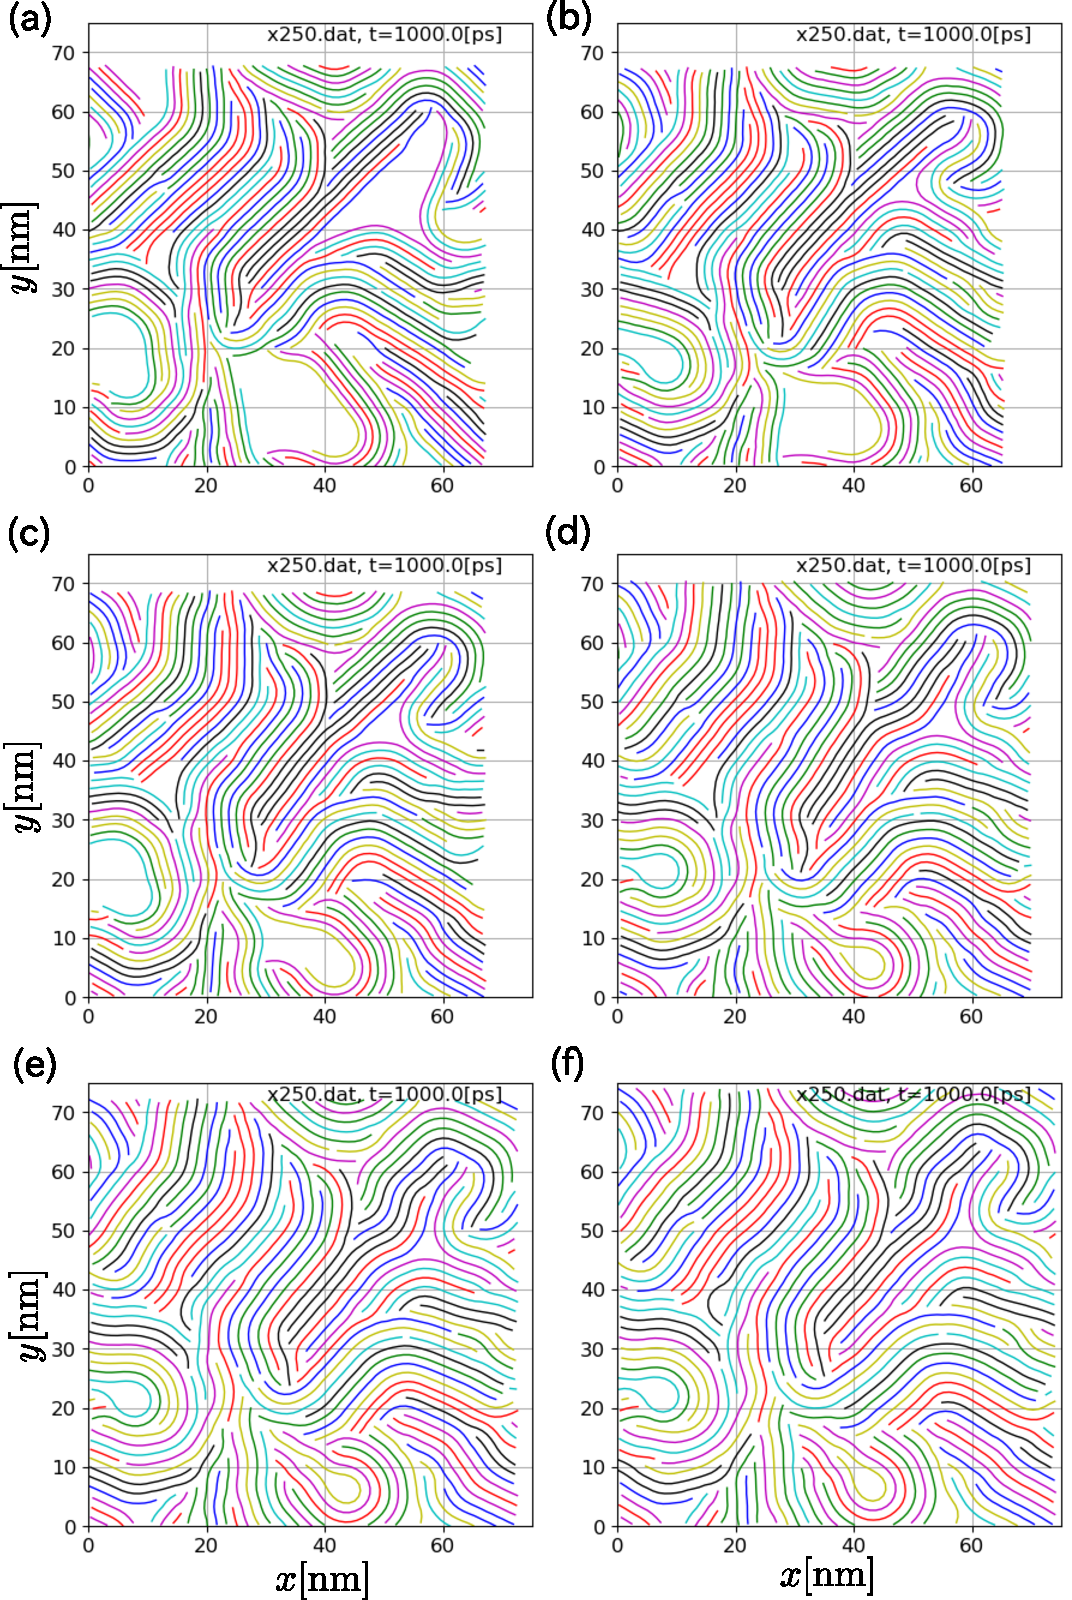
\includegraphics[width=0.9\linewidth]{Figs/fig4.eps} 
	\end{center}
	\caption{
		温度(300K),体積,化学ポテンシャル一定での緩和.
		(a)は緩和開始時の状態,(b),(c),(d)は各々の図に示された
		無次元化化学ポテンシャルで緩和後の状態.
	} 
	\label{fig:fig4}
\end{figure}
%--------------------
\begin{figure}[h]
	\begin{center}
%	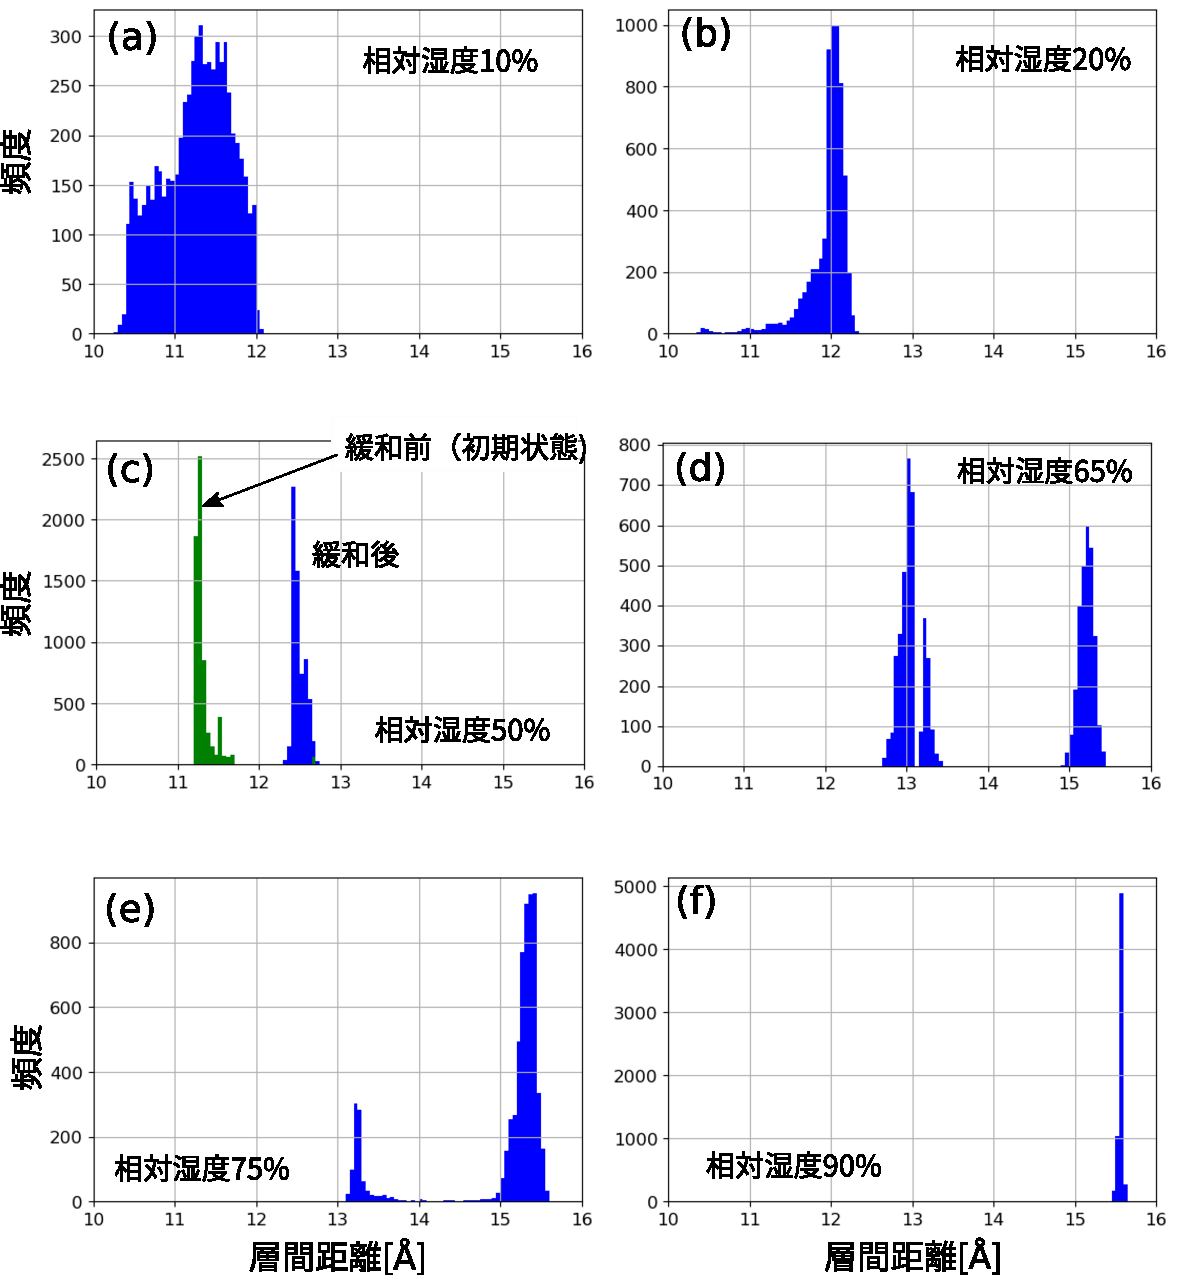
\includegraphics[width=0.7\linewidth]{Figs/fig5.eps} 
	\end{center}
	\caption{
		緩和過程におけるエネルギーの推移($\bar{\mu}=0.3の場合$).
	} 
	\label{fig:fig5}
\end{figure}
%--------------------
\begin{figure}[h]
	\begin{center}
%	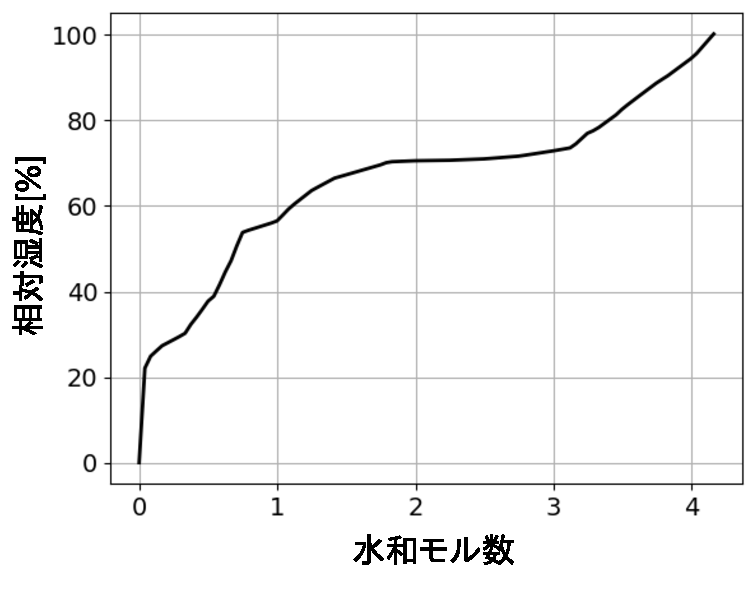
\includegraphics[width=0.9\linewidth]{Figs/fig6.eps} 
	\end{center}
	\caption{
		水和層厚さの頻度分布.(a)は緩和開始時,(b),(c),(d)は
		各々の図に示された無次元化化学ポテンシャルでの緩和後.
	} 
	\label{fig:fig6}
\end{figure}
%--------------------
\begin{figure}[h]
	\begin{center}
%	\includegraphics[width=1.0\linewidth]{Figs/fig7.eps} 
	\end{center}
	\caption{
		化学ポテンシャル一定条件での緩和による粘土分子配置と水和層厚分布の変化.
		無次元化化学ポテンシャル$\bar{\mu}=0.1$,初期状態で水分配置に大きなばら
		つきがある場合.
	} 
	\label{fig:fig7}
\end{figure}
%--------------------
\begin{figure}[h]
	\begin{center}
%	\includegraphics[width=0.9\linewidth]{Figs/fig8.eps} 
	\end{center}
	\caption{
		温度(300K),圧力(50MPa),化学ポテンシャル一定での緩和.
		(a)は緩和開始時の状態,(b),(c),(d)は各々の図に示された
		無次元化化学ポテンシャルで緩和後の状態.
		水和エネルギーに単調モデルを用いた場合の結果.
	} 
	\label{fig:fig8}
\end{figure}
%--------------------
\begin{figure}[h]
	\begin{center}
%	\includegraphics[width=0.9\linewidth]{Figs/fig9.eps} 
	\end{center}
	\caption{
		水和層厚さの頻度分布.(a)は緩和開始時,(b),(c),(d)は
		各々の図に示された無次元化化学ポテンシャルでの緩和後.
		それぞれの図は,図\ref{fig:fig8}に示した粘土分子配置
		に対応するもの.
	} 
	\label{fig:fig9}
\end{figure}
%--------------------
